\documentclass[10pt]{article}

%\usepackage[utf8]{inputenc}
\usepackage[english]{babel}
\usepackage{geometry}
\geometry{legalpaper, margin=1in}

\usepackage{amssymb,amsmath}
\usepackage{subfig}
\usepackage{graphicx}
\usepackage{color}
\usepackage{hyperref}
\usepackage{listings}
\usepackage{multicol}

\newenvironment{Figure}
{\par\medskip\noindent\minipage{\linewidth}}
{\endminipage\par\medskip}

\newenvironment{Table}
{\par\medskip\noindent\minipage{\linewidth}}
{\endminipage\par\medskip}

\newenvironment{Gather}
{\par\medskip\noindent\minipage{\linewidth}}
{\endminipage\par\medskip}


\begin{document}

\title{Radiation-Material Interaction Measurments for Monoenergetic Alpha Particles and Gamma Rays}

\author{Department of Nuclear Engineering \\ University of Wisconsin, Madison, WI, USA}
\date{\today}

\maketitle

\begin{abstract}
	Radiation-material interactions are an important topic in many cross disciplinary scientific and engineering fields.  In this paper we discuss the theoretical background, and how it guided our experimental procedure,  for measuring the absorption of $5.486 \ MeV$ $\alpha$-particles in air at standard temperature and pressure, and the absorption coefficients of aluminum and lead for $411.8 \ keV$ $\gamma$-rays.  We measured the mean range for the $\alpha$-particles to be $(4.02 \pm 0.05) \ cm$,  which has a $3.60 \%$ with the expected value of $4.17 \ cm$ \cite{bib:5}.  For the aluminum and lead absorption coefficients, we measured $(0.076 \pm 0.003) \ cm^{2}/g$ and $(0.199 \pm 0.003) \ cm^{2}/g$, respectively.  Which have $17.4 \%$ and $11.2\%$ error with their expected values of $0.092 \ cm^{2}/g$ and $0.224 \ cm^{2}/g$ \cite{bib:4}. Ultimately, we provide several experimental design improvements that could be made to improve these results.
\end{abstract}

\begin{multicols}{2}

\section{Introduction}
All claims in this introduction are reference to (\cite{bib:1}, \cite{bib:2} and \cite{bib:3}). \par

Understanding how radiation can be absorbed by a material is a crucial component in modern science. Whether you are an experimental particle physicist, a nuclear engineering or a doctor performing proton therapy; knowing what material to use to shield a radioactive environment can be the difference between a good and bad experiment, or in more extreme cases, life and death. For the student, however, it is similarly important they understand how various radiation absorption parameters are measured for different materials.  This will provide them with a better understanding of these values when they encounter them in experiments of their own.  \par 

For most energetic $\alpha$-particles, a few $cm$ of air, at standard temperature and pressure (stp), has sufficient stopping power to block most of the radiation.  The stopping power ($S$) of a medium is defined as the energy lost by a particle per unit path length, as shown in Equation \ref{stp}.  Similarly, $S$ relates to the stopping range ($R$) by Equation \ref{rng}.

\begin{equation}
	S = \langle - \frac{dE}{dx} \rangle \label{stp}
\end{equation}

\begin{equation}
	R = \int_{0}^{R} dx = \int_{0}^{E_{0}} \frac{dE}{ \langle -\frac{dE}{dx} \rangle}
	\label{rng}
\end{equation}

It is worth noting that when one observes the number of $\alpha$-particles emitted by a source as a function of the detector's distance from that source, the number will remain constant up to a particular distance.  Then, if the source is moved further away, the detector will observe a precipitous drop in the number of $\alpha$-particles.  This region of diminishing counts provides another interpretation for the $\alpha$-particle's range.  In this formulation, the range can be understood as the distance between the detector and the source at which the number of $\alpha$-particles detected has dropped by a factor of 2. \par 

For distances below this range, the stopping power of particles with a specific charge state, in a particular medium, can be described by the \textit{Bethe} formula.

\begin{gather}
-\frac{dE}{dx} \approx \frac{4\pi e^{4}z^{2}}{m_{0}v^{2}}NZ \ln \left(\frac{2m_{0}v^{2}}{I}\right) \label{beth}
\end{gather}  

In this equation, $v$ and $ze$ are the velocity and charge of the primary particle, $N$ and $Z$ are the number density and atomic number of the atoms in the absorbing medium, $m_{0}$ is the electron rest mass, $e$ is the electronic charge and $I$ is the experimentally measured average excitation and ionization potential of the absorber.  This is only an approximate expression, there is a relativistic correction not included here since we will be dealing only with non relativistic $\alpha$-particles. \par 

As opposed to $\alpha$-particles, $\gamma$-rays are capable of penetrating much more deeply into most materials.  Their interaction with a material is a consequence of three primary interactions: (1) photoelectric absorption, (2) Compton scattering and (3) pair production.  The sum of the probabilities of these three interactions is the probability per unit path length that an individual $\gamma$-ray photon will be removed from the beam path.  This value is called the \textit{linear attenuation coefficient} or $\mu$.  The number of transmitted $\gamma$-ray photons through a medium can then be described by the following exponential equation, where $I_{0}$ is the number of photons detected without an absorbing medium present, and $t$ is the total path length.

\begin{equation}
	I = I_{0} e^{-\mu t} \label{abs_coef}
\end{equation}   

The natural logarithm of equation \ref{abs_coef} gives a linear relationship between the log of $\gamma$-ray counts and the the material's absorption coefficient ($\mu$)

\begin{equation}
	\ln \left(I\right) = \ln \left(I_{0}\right) -\mu t \label{log_coeff}
\end{equation}

In this paper, we will use our understanding of how radiation interacts with a material to perform two separate experiments.  First, we will consider the absorption of $5.486 \ MeV$ $\alpha$-particles in dry air at stp.  In the second experiment, we measure the absorption coefficient of $411.8 \ keV$ $\gamma$-rays in both aluminum and lead.  In the following sections of this paper, we will describe our experimental approach for both experiments, we will present the results of those exerpiments, and finally, we will discuss the significance and the error of those results as they compare to previously measured values.  \par 

\section{Approach} \label{appr}
In this section, we describe our experimental procedure for measuring the stopping power and mean range of $5.486 \ MeV$ $\alpha$-particles in air.  We then discuss our experimental procedure for measuring the absorption coefficients of $411.8 \ keV$ $\gamma$-rays in both aluminum and lead. 

\subsection{Alpha Particle Experiment} \label{alf_apprch}

To measure the count rate of $\alpha$-particles, we used a silicon-diffused junction detector with an energy resolution of 10-13 keV.  The detector was mounted in a vacuum chamber and biased with a high voltage power supply.  A diagram of the vacuum chamber setup is shown in figure \ref{vacc_diag}.  The signal from the detector was then fed into a preamplifier to amplifier setup, whose output was continuously observed on an oscilloscope throughout the duration of the experiment.  All spectral measurements were made using a multichannel analyzer (MCA).  A diagram of the electronics setup is shown in figure \ref{elec_diag}.

\begin{Figure}
	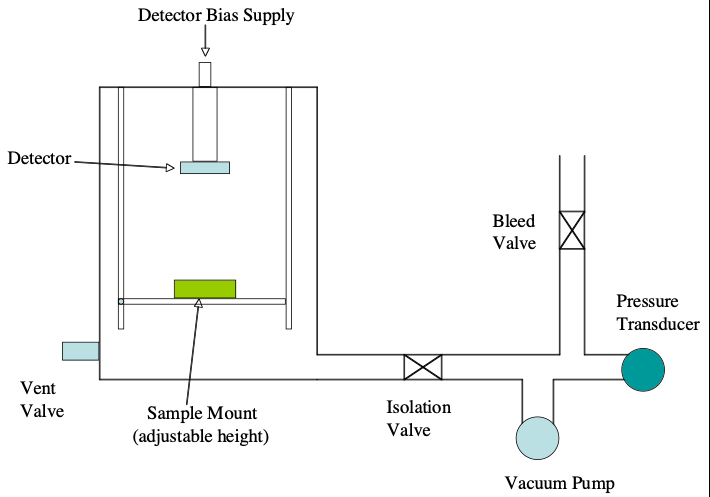
\includegraphics[width=\textwidth,keepaspectratio]{vacc_diag.png}
	\captionof{figure}{Here we present a diagram of the alpha particle stopping energy experimental setup inside the vacuum chamber.  \label{vacc_diag}}
\end{Figure} 

\begin{Figure}
	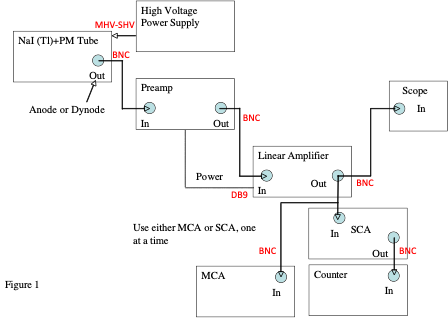
\includegraphics[width=\textwidth,keepaspectratio]{elec_diag_2.png}
	\captionof{figure}{Here we present a diagram of the electronics setup used in the alpha particle stopping energy experiment.  \label{elec_diag}}
\end{Figure} 

We used the chamber air pressure as a proxy for the detector's distance from the source.  We were then able to calculate the effective distance ($d_{eff}$) between the source and the detector using the following equation: 


\begin{equation} 
d_{eff} = \frac{1}{\rho_{stp}}\frac{P(MW)_{air}}{RT}d \label{deff}
\end{equation}

Where $\rho_{stp}$ is the density of air at standard temperature and pressure ($1.2 \ mg/cm^{3}$), $P$ is the measured pressure in the chamber, $(MW)_{air}$ is the molecular weight of air ($0.02897 \ kg/mol$), R is the gas constant ($8.314 \ \frac{J}{K \cdot mol}$), T is the temperature in the room ($293 \ K$) and d is the measured distance between the detector and the source ($5.5 \ cm$). \par

The pressure within the chamber was measured using a pressure sensor readout on a digital voltmeter.  When fully vented, the pressure sensor was recorded at 7440 $mV$.  Taking the pressure of a fully vented chamber to be 760 $Torr$, we can relate the voltage reading to pressure by multiplying the reading on the voltmeter by a factor of 0.102 $Torr/mV$.  We then determined a lower pressure bound for our experiment by running the roughing pump until the voltage reading stabilized at a minimum value of 5.7 $mV$, corresponding to a chamber pressure of 0.6 $Torr$. \par

Then, to properly calibrate the electronic setup, we vented the chamber and moved the alpha source to be as close to the detector as possible.  At atmospheric pressure, we observed the detector signal from the preamplifier output on the oscilloscope, increasing the detector biasing voltage until we observed a tolerable signal-to-noise ratio.  We then observed the signal on the oscilloscope from the amplifier output, increasing the coarse and fine gain until our signal peaked around 5 $V$.  The resulting instrument settings of this calibration analysis are shown in table \ref{elec_set}, and they were unchanged throughout the duration of the experiment. 

\begin{Table}
	\centering
	\begin{tabular}{|l|l|}
		\hline
		\multicolumn{2}{|c|}{Electronic Settings} \\ \hline
		Biasing Voltage     & 30 V     \\ \hline
		Coarse Gain         & 100      \\ \hline
		Fine Gain           & .85      \\ \hline
		Net Gain            & 85       \\ \hline
	\end{tabular}
	\captionof{table}{Electronics settings in alpha particle stopping energy experiment. \label{elec_set}}
\end{Table}

Knowing the mean range of a 5.486 $MeV$ alpha particle source is expected to be around 4 $cm$ at stp (citation), we positioned our source 5.5 $cm$ away from the detector and verified on the oscilloscope that we did not observe any measured signal.  We then closed the vacuum chamber and let the roughing pump run until we reached our low pressure equilibrium.  We then recorded the voltage on the voltage reader and took a spectrum using the MCA, letting it collect data for 120 seconds.  From the spectrum, we recorded the pulse peak channel, the full width at half maximum (FWHM) in channel number and gross counts with corresponding error.  We then opened the bleed valve slightly and allowed the pump to reach a new equilibrium pressure.  This step usually required us to modify the bleed valve opening until we reached the desired incremental pressure increase.  We then recorded the pressure sensor voltage and took another spectrum for 120 seconds, recording the same spectral data mentioned above.  We repeated this process until the gross counts began to drop precipitously.  We then performed the same measurements but in finer pressure increments until a full data set across a range of chamber pressures had been acquired.

\subsection{Gamma Ray Experiment}
In the gamma ray absorption experiment we used the same electronics setup as described in section \ref{alf_apprch}, and depicted in figure \ref{elec_diag}.  Though we used a NaI(Ti) scintillation detector for gamma ray detection instead of the silicon-diffused junction detector, and the radiation source and detector were mounted inside a lead pig instead of a vacuum chamber.  The gamma ray source was an irradiated $^{198}Au$ foil, positioned below a lead collimator.  We used a collimated gamma ray beam so as to prevent the detection of scattered $\gamma$-rays (or other photonic noise) in the absorbing medium.  In between the collimator opening and the NaI(Ti) detector was an area for stacking various thicknesses of absorbers.  The mounting configuration is shown in figure \ref{mount_diag}

\begin{Figure}
	\centering
	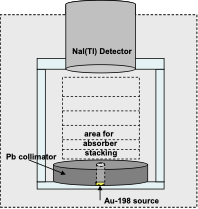
\includegraphics[width=.75\textwidth,keepaspectratio]{mount_diag.png}
	\captionof{figure}{Here we present a diagram of the detector/source mounting system used in the gamma ray absorption experiment. \label{mount_diag}}
\end{Figure} 

We began with a single spectrum with the $^{198}Au$ source in place and no absorber present.  This allowed us to set a region of interest (ROI) in between channels 355 and 440, spanning the $\gamma$ peak.  This ROI remained unchanged throughout the duration of the experiment and was used to determine the gross counts in each spectra.  We then recorded the spectra with various thicknesses of aluminum and lead absorbers, never mixing the two absorbing materials.  Then, we took a background spectra for each absorbing material thickness, but this time without any source present.  From this data, we were able to determine the gamma ray absorbing coefficients of both materials.


\section{Results} \label{res}

In this section we discuss the analysis of all relevant data from the two experimental procedures discussed in section \ref{appr}.  We include brief descriptions of all derived quantities with corresponding errors.  First we consider the alpha particle stopping energy experiment, and then we go on to look at the gamma ray absorption experiment.

\subsection{Alpha Particle Results} \label{res_alpha}

In figure \ref{alph_spec} we show a collection of spectra of alpha particle counts as a function of MCA channel number at various chamber pressures. The chamber pressure is shown in the figure's legend for each spectrum color.  From this figure we see qualitatively that as chamber pressure increases, peak channel decreases and peak width increases.  This remains true until the high pressure spectral peaks approach the lower discriminator for the MCA, at which point the peak width exceeds the observational window of the MCA.  This high pressure boundary begins around 530 $Torr$ and leads to an observed drop in peak width.  This qualitative behavior is best demonstrated in figure \ref{alph_decay_feat}, where the top plot depicts peak channel number and the bottom plot depicts peak width, both as a function of chamber pressure.  In both figures, the error on the measurements are smaller than the plotting point size.

\begin{Figure}
	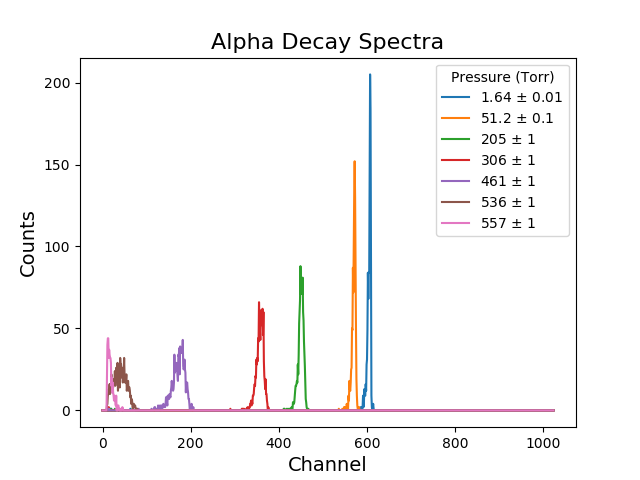
\includegraphics[width=\textwidth,keepaspectratio]{spectra_samples.png}
	\captionof{figure}{Here we present a few sample spectra of the detected alpha particle decays at an assortment of pressures. \label{alph_spec}}
\end{Figure} 

\begin{Figure}
	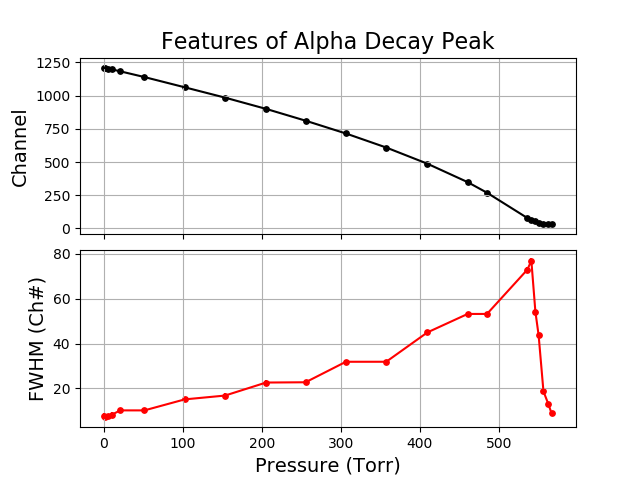
\includegraphics[width=\textwidth,keepaspectratio]{alf_peak_feat.png}
	\captionof{figure}{Both of the above plots show particular features of the alpha decay peaks as a function of chamber pressure. (Top) is plotted the channel at which the alpha decay peak occurred, (Bottom) is plotted the FWHM in channel number of the alpha decay peak.  \label{alph_decay_feat}}
\end{Figure} 

When at the lower pressure boundary of $(0.6 \pm 0.1) \ Torr$, the spectral peak occurs at channel $(1211\pm1)$.  If we assume that at such low pressure the $\alpha$-particles undergo no collisions, then we can approximate that channel $(1211 \pm 1)$ would correspond to the known mean energy of the alpha source ($5.486 \ MeV$) with an error of $\pm 0.02 \ MeV$ due to the pressure approximation.  This allows us to map peak channel number to the mean energy of the $\alpha$-particles by scaling channel number by a factor of $0.0045$ and mapping chamber pressure to $d_{eff}$ using equation \ref{deff}.  The results of this mapping are shown in figure \ref{alph_energy}, where we have plotted mean alpha particle energy as a function of effective stopping distance.  The red star in the plot marks the peak of the stopping power curve, which will be discussed in the next paragraph.

\begin{Figure}
	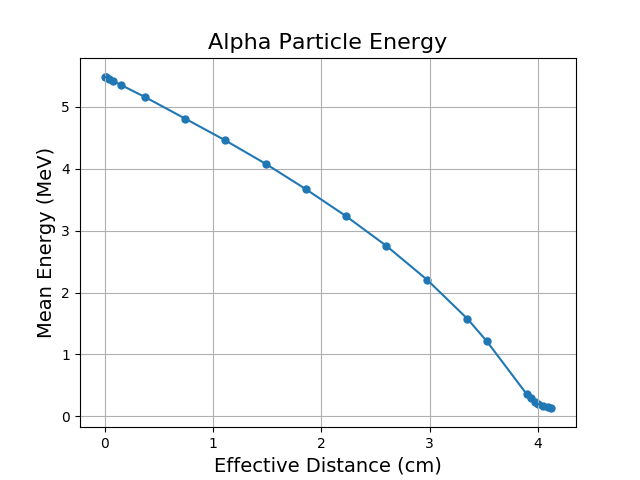
\includegraphics[width=\textwidth,keepaspectratio]{alph_energy.png}
	\captionof{figure}{Here we present alpha particle energy as a function of the effective distance of the emitter source from the detector.  The red star indicates the $d_{eff}$ and mean energy coordinates of the peak stopping power. \label{alph_energy}}
\end{Figure} 

We then use a 1 dimensional spline interpolation to approximate the mean energy as a function of effective distance in between the measured data points. This allowed us to calculate the stopping power $\langle - \frac{dE}{dx} \rangle$ as a function of mean energy. The resulting calculation is shown in figure \ref{stop_pwr}, where we have marked the peak of the curve with a red star.  The stopping power error is a combination of the measurement propagation error and the numerical error of the spline interpolation added in quadrature. 

\begin{Figure}
	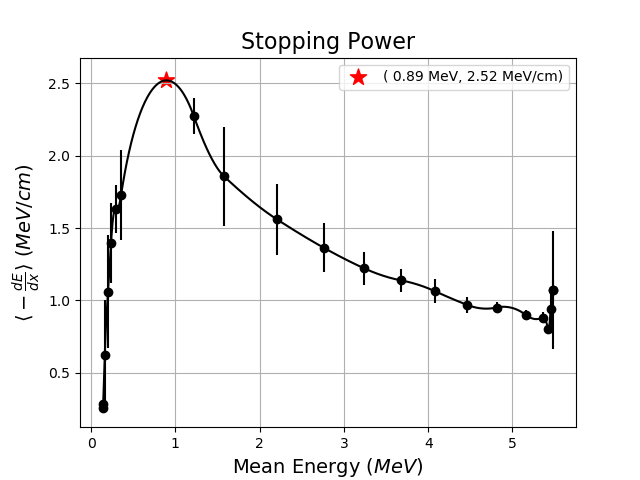
\includegraphics[width=\textwidth,keepaspectratio]{stop_pwr.png}
	\captionof{figure}{Here we present the stopping power of the emitted $\alpha$-particles as a function of effective distance from the alpha emitter to the detector.  The red star indicates the peak stopping power, with the corresponding coordinates listed in the legend. \label{stop_pwr}}
\end{Figure} 

Lastly, we determined the mean range by considering the plot of alpha count rates as a function of effective distance, shown in figure \ref{alph_decay_cnts}.  In this plot we define $d_{eff}^{*} = 3.66 \ cm$ as the effective distance at which we observe the peak stopping power of the $\alpha$-particles.  To then calculate the mean range we first calculated the average count rate for $d_{eff} < d_{eff}^{*}$ and divided it by $2$, shown in blue in figure \ref{alph_decay_cnts}.  We then performed a linear fit to the count rate for $d_{eff} > d_{eff}^{*}$.  Finally, we determined the effective distance at which the linearly fit  of the data for $d_{eff} > d_{eff}^{*}$ intersects with a count rate that is half the mean count rate for $d_{eff} < d_{eff}^{*}$.  This calculation is show in red in figure \ref{alph_decay_cnts}.  This later value we took to be the mean range, and was determined to be $(4.02 \pm 0.05 ) \ cm$.

\begin{Figure}
	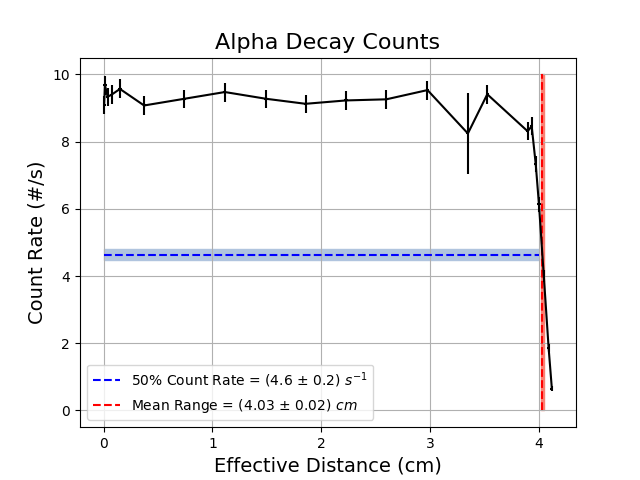
\includegraphics[width=\textwidth,keepaspectratio]{alf_peak_cnts.png}
	\captionof{figure}{Here we present the alpha decay count rate as a function of the detector's effective distance from the source.  Included in the plot is our calculation of the mean range of the $\alpha$-particles (shown in red) as measured when the count rate drops to 50$\%$ its operational rate (shown in blue).  The shaded regions in the plot represent error in our measurements.   \label{alph_decay_cnts}}
\end{Figure} 

\subsection{Gamma Ray Result} \label{res_gamma}

In Figure \ref{gam_spec} we have shown a few spectra taken in the gamma ray absorption experiment.  In Figure \ref{gam_spec_back} we show the background spectrum, taken without any radioactive source present in the detection chamber.  Figure \ref{gam_spec_noShd} is a spectrum taken with the $^{198}Au$ source present, but with no absorbing material between the source and the detector.  Figure \ref{gam_spec_Al} shows a spectrum with an aluminum absorber of thickness $4.2 \ g/cm^{2}$ present, and Figure \ref{gam_spec_Pb} is a spectrum with a $4.568 \ g/cm^{2}$ thick lead absorber present.  In each figure, the ROI is indicated in red between channel numbers 355 and 440. \par
	
In Figures \ref{Al_gam} and \ref{Pb_gam} we show gamma ray count rates as a function of absorber thickness for both aluminum and lead absorption, respectively. Then, from equation \ref{log_coeff}, we see that if we take the natural log of the count rates and perform a linear regression analysis against absorber thickness, then the negative slope of the resulting line is our measured absorption coefficient ($\mu_{Al,Pb}$) for each material's response to a $.412 \ MeV$ gamma ray source.  These linear fits and the corresponding absorption coefficients are plotted with our data in Figures \ref{Al_shd} and \ref{Pb_shd} for aluminum and lead absorption, respectively.

\begin{Figure}
	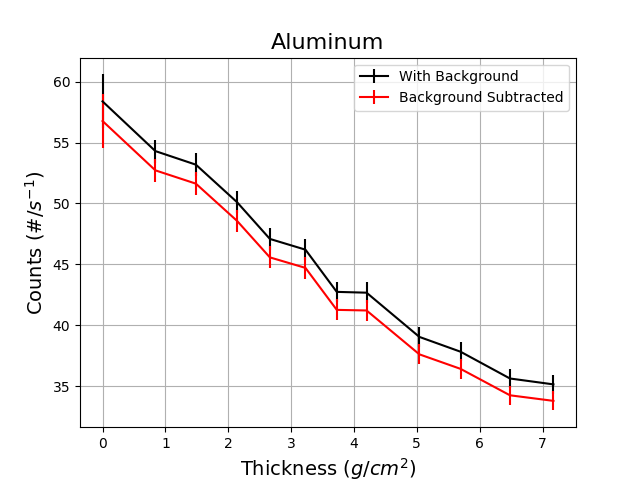
\includegraphics[width=\textwidth,keepaspectratio]{Aluminum_bckg.png}
	\captionof{figure}{Here we present the count rate as a function of absorber thickness for the aluminum absorber.  The count rate without background subtraction is shown in black and with the subtraction is shown in red.   \label{Al_gam}}
\end{Figure} 

\begin{Figure}
	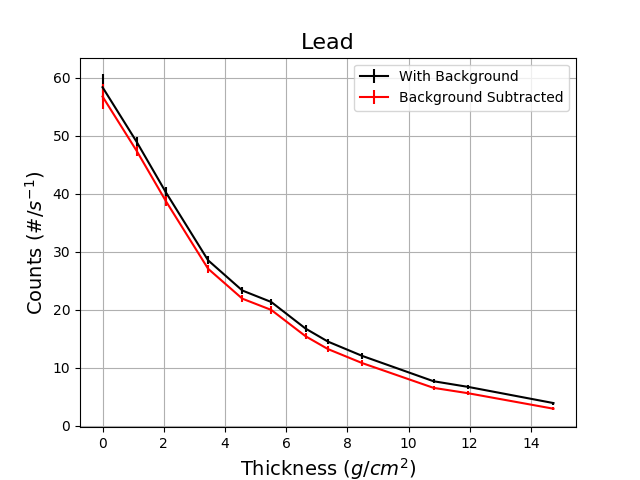
\includegraphics[width=\textwidth,keepaspectratio]{Lead_bckg.png}
	\captionof{figure}{Here we present the count rate as a function of absorber thickness for the lead absorber.  The count rate without background subtraction is shown in black and with the subtraction is shown in red.   \label{Pb_gam}}
\end{Figure} 

\begin{Figure}
	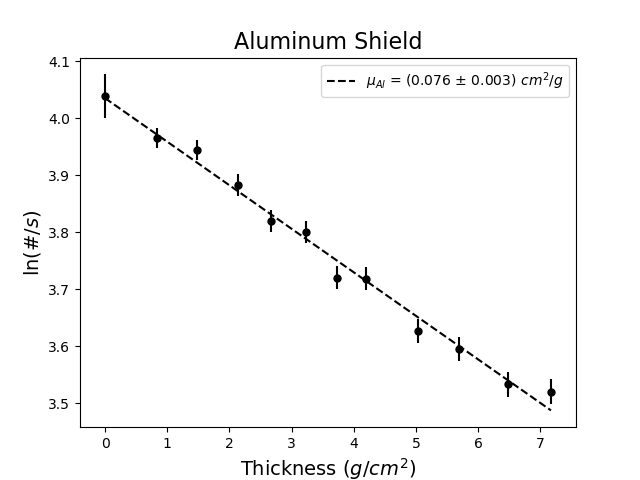
\includegraphics[width=\textwidth,keepaspectratio]{Aluminum_shield.png}
	\captionof{figure}{Here we present the natural log of the count rate as a function of absorber thickness for the aluminum absorber, with a linear regression analysis depicted by the dashed line.   \label{Al_shd}}
\end{Figure} 

\begin{Figure}
	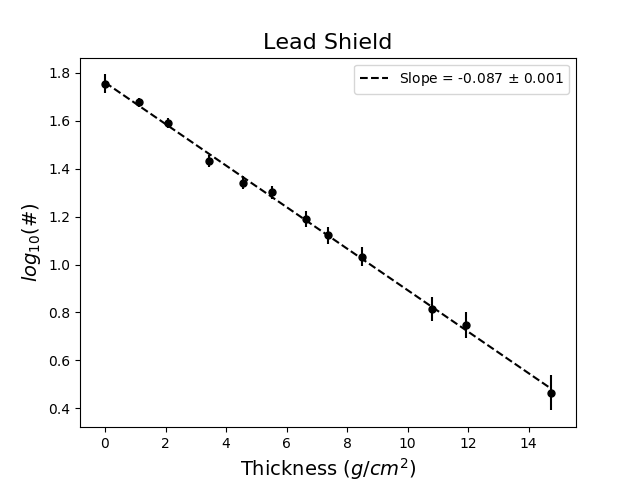
\includegraphics[width=\textwidth,keepaspectratio]{Lead_shield.png}
	\captionof{figure}{Here we present the natural log of the count rate as a function of absorber thickness for the lead absorber, with a linear regression analysis depicted by the dashed line.   \label{Pb_shd}}
\end{Figure} 

\end{multicols}

\begin{figure}
\begin{tabular}{cccc}
	\subfloat[Background radiation spectra taken without a source. \label{gam_spec_back}]{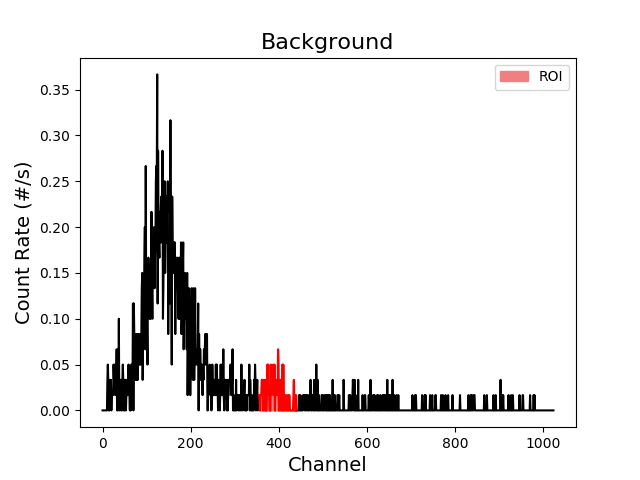
\includegraphics[width=.5\textwidth, keepaspectratio]{bckgrnd.png}} &
	\subfloat[Gamma decay spectra taken without a shield. \label{gam_spec_noShd}]{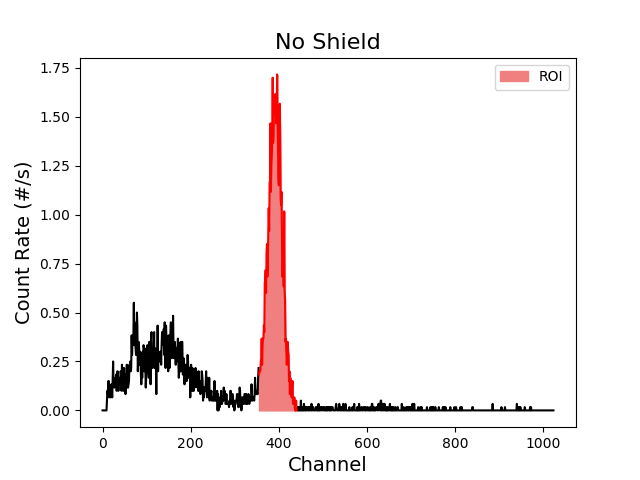
\includegraphics[width=.5\textwidth, keepaspectratio]{no_shield.png}} \\
	\subfloat[Gamma decay spectra with an Aluminum shield. \label{gam_spec_Al}]{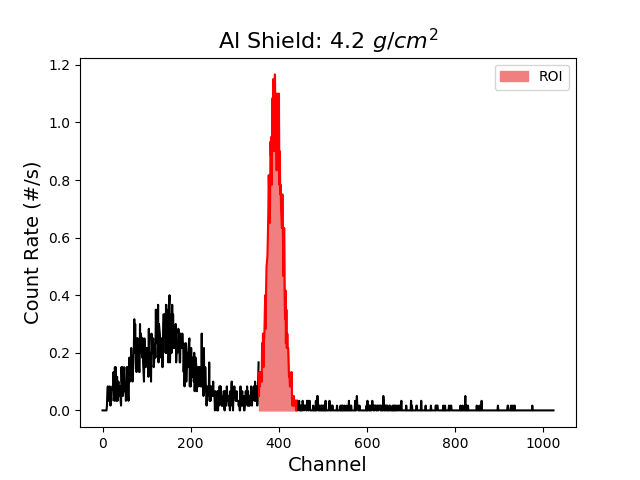
\includegraphics[width=.5\textwidth, keepaspectratio]{Al_shield.png}} &
	\subfloat[Gamma decay spectra with a Lead shield. \label{gam_spec_Pb}]{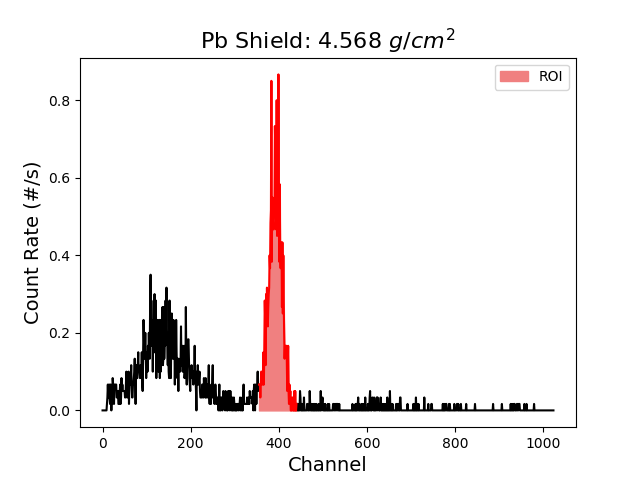
\includegraphics[width=.5\textwidth, keepaspectratio]{Pb_shield.png}}
\end{tabular}
\caption{Above are three spectra taken with a $^{198}Au$ gamma ray source and one spectra taken without any source. \label{gam_spec}}
\end{figure}

\begin{multicols}{2}


\section{Discussion} \label{dis}
In this section we will provide explanations for the results shown in section \ref{res}.  We will compare the measurements we derived from our data with their expected values, and discuss any sources of error in our experiments.

\subsection{Alpha Particle Discussion} \label{dis_alpha}
In Figure \ref{alph_decay_feat} we saw that the spectral alpha peaks dropped in channel number and rose in channel width due to an increase in chamber pressure.  This is best described by the Coulomb collisions between the charged $\alpha$-particles and the orbital electrons of the air molecules in the chamber.  Since collision frequency rises with chamber pressure, the $\alpha$-particles lose more kinetic energy due to collisions as a function of increasing pressure.  This corresponds with a decreasing channel peak on the MCA.  Similarly, as more collisions take place, the energy spread of the $\alpha$-particles widens as the $\alpha$-particles begin to thermalize with the residual air inside the chamber, contributing to a rising FWHM as a function of chamber pressure. \par                 

In figure \ref{stop_pwr} we see the steep rise in stopping power for low energy $\alpha$-particles, which corresponds to the deeply penetrating $\alpha$-particles in figure \ref{alph_energy}.  This region demonstrates qualitatively the tendency for low energy $\alpha$-particles to neutralize after picking up charged electrons from the surrounding air molecules.  Though after the peak stopping power, which occurs at ($0.89 \pm 0.05$) $MeV$, the stopping power starts to decrease as $\frac{1}{E}$ as described by equation \ref{beth}, which corresponds to mean alpha particle energies with an effective penetrating distance $\lesssim d_{eff}^{*}$. \par 

For our determination of the mean range of $5.486 \ MeV$ $\alpha$-particles in air, we measured $(4.02 \pm 0.05) \ cm$, which, when compared to the expected value of $4.17 \ cm$, as measured in \cite{bib:5}, gives our measured value an error of $3.60 \%$. \par  

Though our percent error is small, the expected value is outside of our error window.  This would indicate a small systematic error in the experiment.  Possible sources of this error are most likely attributed to our treatment of chamber pressure as a proxy for effective distance.  If we were to conduct the experiment again, we would put additional care to properly calibrate our conversion from voltage on the pressure sensor to pressure.  Additional sources of error might include the deviations of temperature, humidity and pressure in the room from stp, since none were parameters we measured. 

\subsection{Gamma Ray Discussion}

The expected absorption coefficients of aluminum and lead are provided by \cite{bib:4}.  For aluminum, we measured an absorption coefficient of $(0.076 \pm 0.003) \ cm^{2}/g$, which has a $17.4 \%$ error when compared to the expected value of $0.092 \ cm^{2}/g$.  For lead, we measured an absorption coefficient of $(0.199 \pm 0.003) \ cm^{2}/g$, which has an $11.2 \%$ error compared to the expected value of $0.224 \ cm^{2}/g$. \par

These results have a relatively larger percentage of error than the $\alpha$-particle experiment, and the expected values are outside the error windows of both measurements.  Therefore, we again expect some systematic error in our experiment.  One issue may have been in how we measured the background $\gamma$ radiation, which was to block the collimated opening for the $\gamma$-rays with a lead pin.  It may be prudent in the future to remove the source entirely before taking the background measurements.  We also may benefit from a deeper collimator, which would further reduce the amount of scattered noise from the the absorbing material.  Similarly, we could fit the data to a corrected model such as that shown in equation \ref{corr}, where $B\left(t, E_{\gamma}\right)$ is known as the \textit{buildup factor}, which represents the attenuation of the $\gamma$-ray beam due to secondary $\gamma$ emissions in the absorbing material.

\begin{equation}
	\frac{I}{I_{0} } = B\left(t, E_{\gamma}\right) e^{-\mu t} \label{corr}
\end{equation}

Lastly, we may again attribute some amount of error to the deviation of the lab's temperature, humidity and pressure compared to stp.

\section{Summary}

In this lab we successfully measured the stopping power and mean range of $5.486 \ MeV$ $\alpha$-particles in air by measuring the count rate spectra at a set of differing chamber pressures with a silicon-diffused junction detector.  We also measured the absorption coefficients of aluminum and lead for $411.8 \ keV$ $\gamma$-rays by stacking the two absorbing materials between a collimated $\gamma$-ray source and a NaI(Ti) scintillation detector.  In the former experiment, we measured a mean range of $(4.02 \pm 0.05) \ cm$, which has a $3.60 \%$ with the expected value of $4.17 \ cm$ \cite{bib:5}.  In the later experiment, we found absorption coefficient for aluminum and lean to be $(0.076 \pm 0.003) \ cm^{2}/g$ and $(0.199 \pm 0.003) \ cm^{2}/g$, respectively.  Which have $17.4 \%$ and $11.2\%$ error with their expected values of $0.092 \ cm^{2}/g$ and $0.224 \ cm^{2}/g$ \cite{bib:4}.  While our results may be lacking in accuracy, we think with a few changes to the experimental design, as discussed in section \ref{dis}, these results can be improved.  Though ultimately, we feel as though we have demonstrated a reasonable experimental method for performing such measurements. 

\end{multicols}

\newpage

\begin{thebibliography}{99}
\bibitem{bib:1} Knoll, Glenn F. {\it Radiation Detection and Measurement}, 3rd edn. Wiley, 2010.
\bibitem{bib:2}Choy, Jen. ``Lecture-08 Radiation-Matter Interactions Part II.'' Nuclear Engineering 427. 28 Oct. 2019, Madison, WI.
\bibitem{bib:3} Choy, Jen. ``Lecture-09 Radiation-Matter Interactions Part II.'' Nuclear Engineering 427. 4 Nov. 2019, Madison, WI.
\bibitem{bib:4} ``X-Ray Mass Attenuation Coefficients - Table 3.'' {\it NIST}, \\ https://physics.nist.gov/PhysRefData/XrayMassCoef/tab3.html
\bibitem{bib:5} {\it Physical Measurement Laboratory}, physics.nist.gov/PhysRefData/Star/Text/ASTAR.html.
\end{thebibliography}

\newpage

Author:  Michael Gerard \\

Partner: Thomas Adams, Nicholas Anderson



\end{document}